\documentclass{article}
\usepackage[margin=2cm]{geometry}
\usepackage{graphicx}
\usepackage[pages=some]{background}
\usepackage{titling}
\usepackage{tabularx}
\usepackage{tikz}
\usepackage{forest}
\usepackage{float}
\usepackage{subcaption}
\usepackage{amsmath}
\usepackage{amssymb}
\usepackage{multicol}
\usepackage{float}
\usepackage{tabularx}
\usepackage{array}


\forestset{
  my box/.style={
    draw,
    rectangle,
    rounded corners,
    fill=gray!20, 
    inner sep=6pt,
    minimum width=3cm % Adjust the width as needed
  }
}


\geometry{a4paper}

\backgroundsetup{
    scale=1,
    angle=0,
    opacity=1,
    contents={%
        
\includegraphics[width=\paperwidth,height=\paperheight]{institution_logo.jpg}
    }
}

\newcommand{\subtitle}[1]{
    \posttitle{
        \par\end{center}
        \begin{center}\large#1\end{center}
        \vskip0.5em}
}

\title{ME-415}
\author{Md. Hasibul Islam}
\subtitle{RWFRIGERATION \& BUILDING MECHANICAL SYSTEM}

\begin{document}
\begin{titlepage}
    \centering
    
    {\Huge\bfseries\maketitle}
    \textbf{Arif Hasan Mamun Sir} \\
    \vspace{2cm}
    
\includegraphics[width=8cm]{institution_logo.jpg}
    \vfill
    \vspace*{2cm}
\end{titlepage}

\tableofcontents
\pagebreak
\section{Lecture 01: Concept of refrigeration and its applications} 
\hfill Date: 05/06/2023

\subsection*{Booklist}
1. Ahmadul Ameen (2006), Refrigeration \& Air-conditioning, 
Prentice Hall.\\
2. Hundy, Trott \& Welch, 4th Edition, Refrigeration \& Air conditioning, Butterworth-Heinemann.\\
3. McQuiston, Parker \& Spitler (2005), Heating, Ventilating \& Air conditioning: Analysis \& Design, J. Wiley \& Sons, Inc.\\
4. Stoecker \& Jones (1983), Refrigeration \& Air-conditioning, 
McGraw-Hill, Inc.\\
5. Dossat (1996), Principles of Refrigeration, Prentice Hall.\\
6. McDowall (2007), Fundamentals of HVAC Systems, Elsevier.\\
7. Grondzik, Kwok, Stein \& Reynolds (2010), Mechanical \& 
Electrical Equipment for Buildings, J. Wiley \& Sons, Inc.\\

\subsection{Refrigeration System and Components}
\subsubsection*{Refrigeration}
Refrigeration is a process of reducing and maintaining low temperature of a space or material below the temperature of the surroundings.\\
Alternatively, Refrigeration is the process of removing heat from an enclosed 
space, or from a substance, and rejecting it elsewhere for the 
purpose of lowering the temperature of the enclosed space or 
substance and then maintaining that lower temperature.\\
It is usually done with the aid of a mechanical device (e.g. pump/compressor) using a substance (called a refrigerant) which absorbs heat from low temperature (objects/space) and releases heat to elsewhere at high temperature. 
A refrigerant usually works in two-phase conditions, i.e., liquid and gas, e.g., vapor compression refrigeration system. 

\paragraph*{Refrigeration System:} 
A refrigeration system is a mechanical system designed to remove heat from a space or substance to lower its temperature. It operates on the principle of the refrigeration cycle, which involves the compression, condensation, expansion, and evaporation of a refrigerant to transfer heat from a low-temperature region to a high-temperature region. The main components of a typical refrigeration system include a compressor, condenser, expansion valve, and evaporator. 

\paragraph*{Types of refrigeration system:}
\subparagraph{Vapor Compression Refrigeration System}: This widely used system compresses a refrigerant gas, causing it to become hot and high-pressure. It then passes through a condenser where it releases heat and condenses into a liquid. The liquid refrigerant expands through an expansion valve, reducing its pressure and temperature, and evaporates in the evaporator, absorbing heat from the surroundings.

\subparagraph{Vapor Absorption Refrigeration System}: This system uses a mixture of refrigerant and absorbent instead of a compressor to achieve cooling. The mixture circulates through an absorber, generator, condenser, and evaporator. Heat is applied to the generator to separate the refrigerant from the absorbent. The refrigerant vapor then flows to the condenser where it liquefies, and the absorbent is regenerated in the absorber for reuse.

\subparagraph{Vapor Ejection Refrigeration System}: In this system, a primary refrigerant is compressed, condensed, and expanded similar to a vapor compression system. However, a secondary refrigerant is used to cool the primary refrigerant vapor through a heat exchanger. The cooled primary refrigerant is then expanded further to achieve the desired cooling effect.

\subparagraph{Air Cycle Refrigeration}: This refrigeration system uses air as the refrigerant. Compressed air is cooled through an expansion process, causing its temperature to decrease. The cooled air is then used to absorb heat from the desired space or substance, creating a cooling effect.

\subparagraph{Vortex Tube Refrigeration}: A vortex tube refrigeration system utilizes a high-pressure gas stream that enters a tangential nozzle, creating a vortex motion. This vortex separates the gas into hot and cold streams, with the cold stream used for refrigeration purposes.

\subparagraph{Thermoacoustic Refrigeration System}: Thermoacoustic refrigeration systems utilize sound waves and thermal gradients to achieve cooling. The sound waves cause compression and expansion of the gas, creating temperature differences that enable cooling.

\subparagraph{Thermoelectric Refrigeration System}: These systems use the Peltier effect, where an electric current is applied to a junction of two different conductive materials, resulting in a temperature difference. This temperature difference allows for cooling when applied in a refrigeration system.

\subparagraph{Cascade Refrigeration System}: Cascade systems consist of two or more refrigeration cycles working in series. Different refrigerants with varying temperature ranges are used in each cycle, allowing for extremely low temperatures in specific applications.

\subparagraph{Cryogenic Refrigeration}: Cryogenic refrigeration involves the use of extremely low temperatures, typically below -150 degrees Celsius (-238 degrees Fahrenheit), to achieve cooling. These systems are used in applications such as liquefied natural gas (LNG) processing, scientific research, and medical processes.

\subparagraph{Magnetic Refrigeration}: Magnetic refrigeration systems use the magnetocaloric effect, where a magnetic material heats up or cools down when subjected to a magnetic field. By cycling the magnetic field, heat can be absorbed or released, providing cooling without the use of traditional refrigerants.
\vspace{0.5cm}
\subsection{Different Components of Vapor 
Compression Refrigeration System}
\begin{figure}[H]
  \centering
  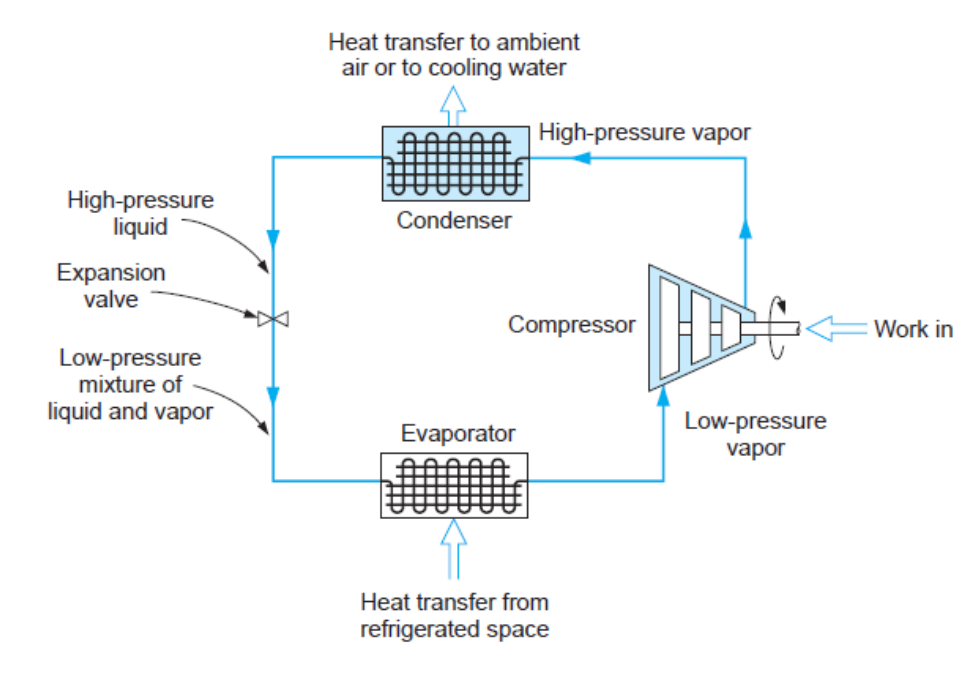
\includegraphics[width=0.75\textwidth]{img/cycle.png}
  \caption{Schematic Diagram of Different Components of Vapor 
  Compression Refrigeration System.}
  \label{fig:components}
\end{figure}
\vspace{0.25cm}

\begin{itemize}
  \item \textbf{Condenser}: The condenser is responsible for removing heat from the refrigerant and converting it from a high-pressure vapor to a high-pressure liquid. It is typically located on the outside of the refrigeration system and uses air or water as a cooling medium. The heat extracted from the refrigerant in the condenser is released into the surroundings.

  \item \textbf{Compressor}: The compressor is the heart of the refrigeration system. Its main function is to increase the pressure and temperature of the refrigerant vapor. The compressor draws low-pressure refrigerant vapor from the evaporator and compresses it to a higher pressure, which raises its temperature as well. This process is crucial for the refrigerant to release heat in the condenser.
  
  
  \item \textbf{Evaporator}: The evaporator is where the refrigerant absorbs heat from the surroundings, typically within the refrigerated space or the object being cooled. As the low-pressure, low-temperature refrigerant enters the evaporator, it absorbs heat from the area and evaporates into a low-pressure vapor. This heat absorption causes the surroundings to cool down. The vapor is then drawn back into the compressor, and the cycle continues.
  
  \item \textbf{Expansion Valve}: The expansion valve is a throttling device located between the condenser and the evaporator. It serves the purpose of reducing the pressure and temperature of the refrigerant as it passes through. The expansion valve creates a pressure drop, allowing the refrigerant to expand rapidly. This expansion results in a decrease in temperature and prepares the refrigerant for the evaporator.
\end{itemize}

\begin{figure}[H]
  \centering
  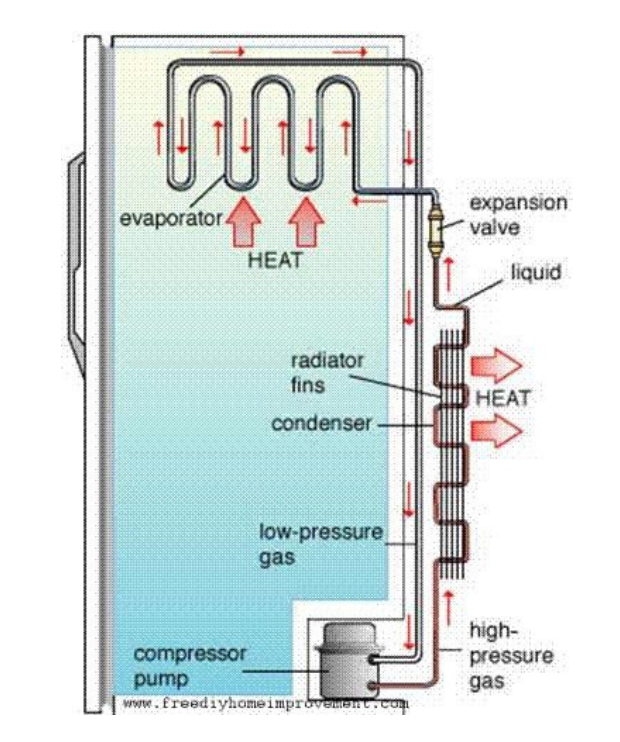
\includegraphics[width=0.55\textwidth]{img/components.png}
  \caption{Different Components of a Refrigeration System.}
  \label{fig:Different Components of a Refrigeration System}
\end{figure}
\vspace{0.25cm}


\begin{figure}
  \centering
  
  \begin{subfigure}{0.45\textwidth}
      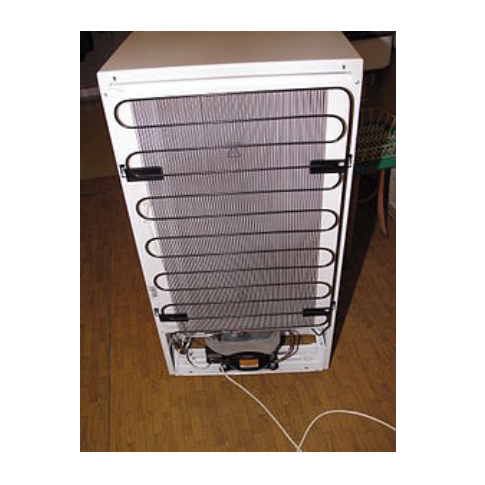
\includegraphics[width=\textwidth]{img/condenser.png}
      \caption{condenser}
      \label{subfig:condenser}
  \end{subfigure}
  \hfill
  \begin{subfigure}{0.45\textwidth}
      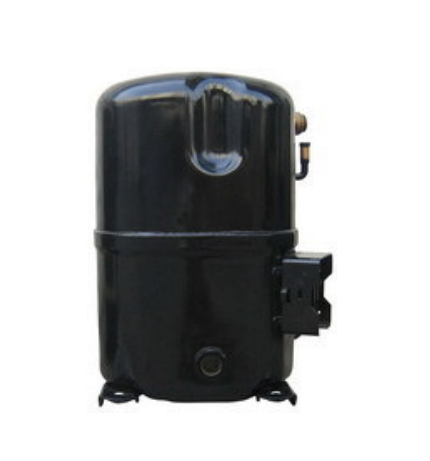
\includegraphics[width=\textwidth]{img/compressor.png}
      \caption{compressor}
      \label{subfig:compressor}
  \end{subfigure}
  
  \vspace{1cm}
  
  \begin{subfigure}{0.45\textwidth}
      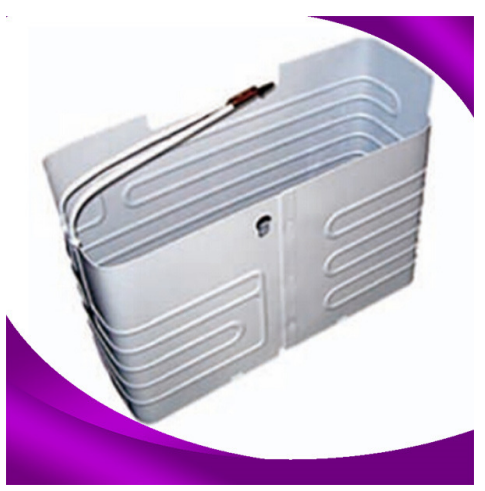
\includegraphics[width=\textwidth]{img/evaporator.png}
      \caption{evaporator}
      \label{subfig:evaporator}
  \end{subfigure}
  \hfill
  \begin{subfigure}{0.45\textwidth}
      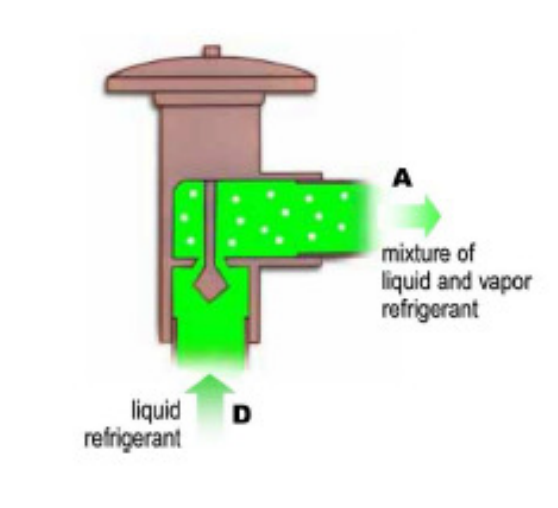
\includegraphics[width=\textwidth]{img/expansion.png}
      \caption{expansion valve}
      \label{subfig:expansion valve}
  \end{subfigure}
  
  \caption{Components of vapour compression refrigeration system}
  \label{fig:four_images}
\end{figure}

\subsection*{Uses of refrigeration system}
\begin{itemize}
  \item Food and Beverage Industry: Storing and preserving perishable items in supermarkets, warehouses, and transport.

  \item HVAC: Cooling and dehumidification in residential, commercial, and industrial buildings.
  
  \item Industrial Processes: Temperature control in manufacturing, equipment cooling, and raw material storage.
  
  \item Cold Chain Logistics: Transporting temperature-sensitive goods, like food, pharmaceuticals, and vaccines.
  
  \item Medical and Healthcare: Storing vaccines, medications, and laboratory samples.
  
  \item Ice Production: Ice manufacturing for commercial use and recreational activities.
  
  \item Research and Scientific Applications: Temperature control in experiments and sample preservation.
\end{itemize}
\vspace{0.5cm}

\subsubsection*{Types of Freezing}
\begin{itemize}
  \item \textbf{Slow freezing: }Slow freezing refers to a method of gradually lowering the temperature of a product over an extended period of time to facilitate freezing. Unlike quick freezing methods that aim for rapid freezing, slow freezing allows for a slower and more controlled freezing process. This method is commonly used in certain food preservation techniques, laboratory research, and some industrial processes. Slow freezing can help maintain the quality, texture, and cellular structure of the product, making it suitable for certain applications where slower freezing is desired or required.
  \item \textbf{Quick Freezing} 
  There are three types of quick freezing systems:
  \begin{itemize}
    \item \textbf{Air Blast Freezing:} Uses high-velocity cold air to rapidly freeze products.
    \item \textbf{Immersion Freezing:} Involves immersing the product in a cold liquid for quick freezing.
    \item \textbf{Indirect Contact Freezing:} Utilizes cold surfaces in direct contact with the product to achieve rapid freezing.
  \end{itemize}
\end{itemize}

\subsubsection*{Industrial Functions of air conditioning}
\begin{itemize}
  \item Temperature control for employee comfort and equipment performance.
  \item Humidity regulation to prevent condensation and protect materials.
  \item Ventilation to remove contaminants and ensure a healthy environment.
  \item Air filtration to maintain air quality and reduce pollutants.
  \item Process and product cooling to optimize manufacturing and storage conditions.
  \item Energy efficiency to minimize costs and maximize cooling effectiveness.
\end{itemize}

\newpage

\section{Lecture 2: Central Air conditioning system}
\hfill Date: 19/06/2023

\subsubsection*{Assignment Notice}
\begin{itemize}
  \item Have to calculate required Ton for air conditioner and a CAD model of room (by autocad or solidworks)
  \item including all the data about room dimension, door specification, dimension, window specification and dimension, slab and wall thickness, heat generating equipment, persons and others 
\end{itemize}

\subsubsection*{Central Air Conditioning System}
A central air conditioning system, also known as a chiller type air conditioning system, is a cooling system that is used to cool large buildings or spaces. It typically consists of a central cooling unit, often referred to as a chiller, that cools water or a refrigerant. The chilled water or refrigerant is then circulated through a network of pipes to various air handling units (AHUs) or fan coil units (FCUs) located throughout the building.

In a chiller type air conditioning system, the chiller unit uses a refrigeration cycle to remove heat from the water or refrigerant, thereby lowering its temperature. The chilled water or refrigerant is then pumped to the AHUs or FCUs, where it passes through heat exchangers. The heat exchangers transfer the coolness from the chilled water or refrigerant to the air, effectively cooling it. The cooled air is then distributed throughout the building via ductwork or individual units, providing a comfortable indoor environment.

Central air conditioning systems offer several advantages, including the ability to cool large spaces efficiently, centralized control and monitoring, and the potential for energy savings through the use of advanced controls and zoning. They are commonly used in commercial buildings, offices, shopping malls, hotels, and other large-scale facilities where cooling requirements are significant.

\begin{itemize}
  \item \textbf{Air Handling Unit (AHU)}: An Air Handling Unit, often referred to as an AHU, is a device used in HVAC systems to condition and distribute air. It typically consists of a fan, heating or cooling elements, filters, and dampers. The AHU pulls in air from the surroundings, treats it by heating or cooling, filters out impurities, and then distributes it to different areas through ductwork.

  \item \textbf{Supply Duct}: A supply duct is a part of the HVAC system responsible for delivering conditioned air from the AHU to different spaces within a building. The supply ducts are connected to the outlets of the AHU and carry the treated air to the desired locations. They are designed to distribute the conditioned air evenly and efficiently throughout the building.
  
  \item \textbf{Return Duct}: A return duct, also known as an exhaust duct or return air duct, is a component of the HVAC system that collects and transports air back to the AHU. It pulls in air from different areas of the building, which may have been circulated through the space or mixed with the indoor air, and directs it back to the AHU for reconditioning.
  \item \textbf{Air Cutter}: An air diffuser or grille designed to direct the flow of conditioned air in a specific pattern or direction. It is typically installed at the outlet of a supply duct or directly on the AHU itself. The air cutter helps to distribute the conditioned air evenly and efficiently throughout the space by controlling the direction, velocity, and spread of the air stream.
\end{itemize}

\section{Lecture 3: Refrigeration Cycle}
\hfill Date: 10/07/2023

\subsubsection*{Problem-01}
A Simple vapor compression refrigeration cycle using R134a as 
refrigerant operates on an ideal vapor compression refrigeration cycle 
between 0.12 and 0.7 MPa. The mass flow rate of the refrigerant is 
0.06 kg/s. Determine:\\
1. The rate of heat removal of the refrigerated space and the 
power input to the compressor \\
2. The rate of heat rejection to the environment \\ 
3. The Coefficient of performance, COP

\subsubsection*{Solution}

\begin{figure}
  \centering
  
  \begin{subfigure}{0.45\textwidth}
      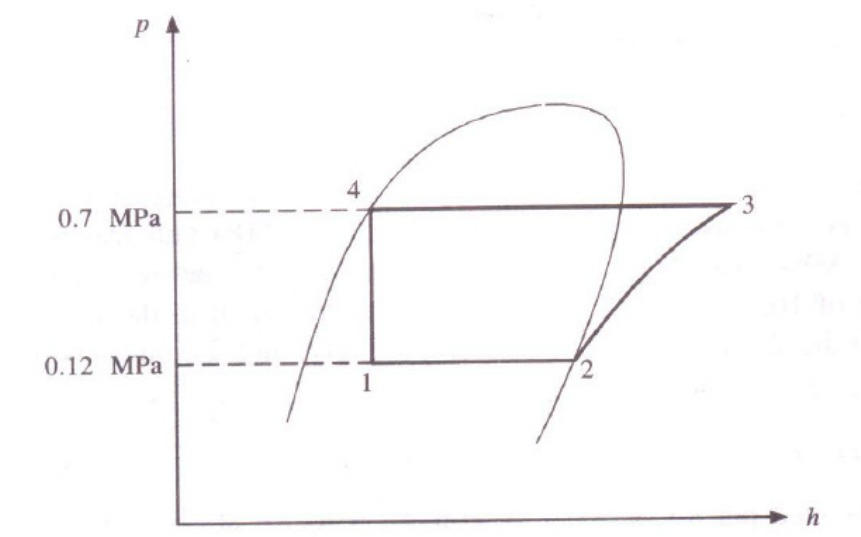
\includegraphics[width=\textwidth]{img/prb-01.jpeg}
      \caption{p-h diagram}
      \label{subfig:p-h diagram}
  \end{subfigure}
  \hfill
  \begin{subfigure}{0.95\textwidth}
      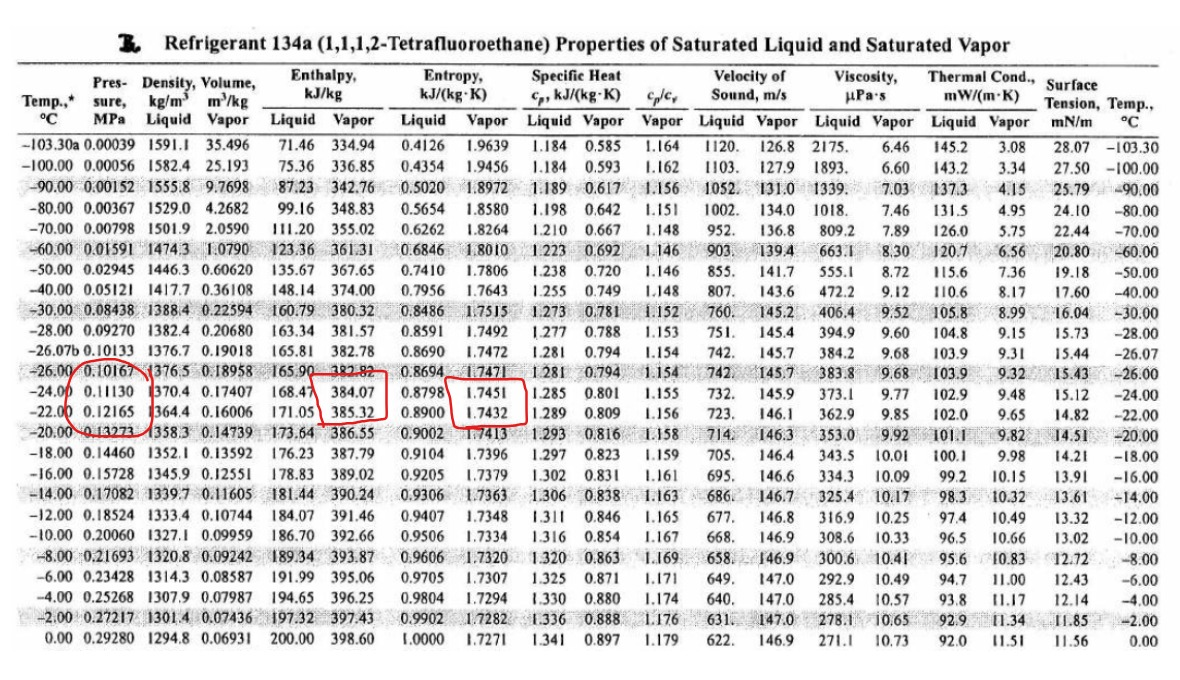
\includegraphics[width=\textwidth]{img/prb-01a.jpeg}
      \caption{Saturated vapor at 0.12 MPa}
      \label{subfig:Saturated vapor at 0.12 MPa}
  \end{subfigure}
  
  \vspace{1cm}
  
  \begin{subfigure}{0.95\textwidth}
      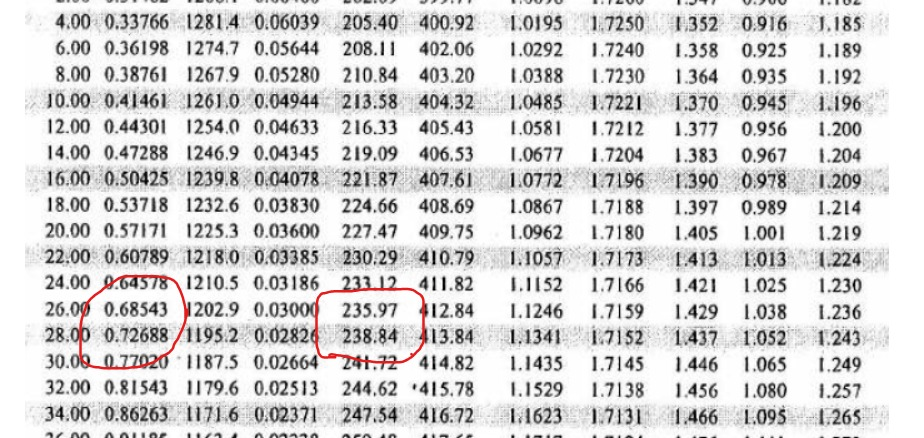
\includegraphics[width=\textwidth]{img/prb-01b.jpeg}
      \caption{Saturated Liquid at 0.7 MPa}
      \label{subfig:Saturated Liquid at 0.7 MPa}
  \end{subfigure}

  
  \caption{Problem-01 Solution}
  \label{fig:problem}
\end{figure}

\begin{figure}[h]
  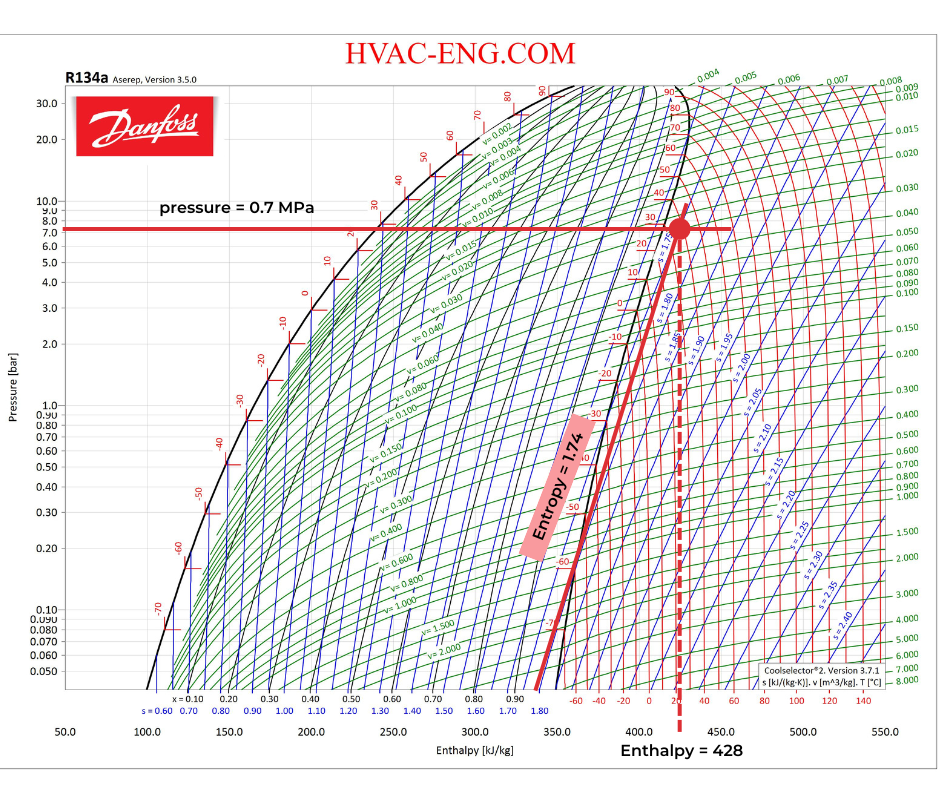
\includegraphics[width=0.95\textwidth]{img/prb-01c.jpeg}
  \caption{Enthaply at s=1.74  and p = 0.7 MPa}
\end{figure}

Here, $P_{cond} = 0.70 $ MPa \\
$P_{eva}$ = 0.12 MPa \\
$\dot{m}$ = 0.06 kg/s \\
For R123a refrigerant,
$h_2=385.43 kJ/kg , h_3 = 428 kJ/kg, h_1 = h_4 = 236 kJ/kg$

(a) 
\begin{align*}
  \text{Refrigering capacity, } Q_2 &= \dot{m}(h_2-h_1) = 8.96 KW \\
  \text{Compressor work, } \dot{W} &= \dot{m}(h_3-h_2) = 2.55 KW 
\end{align*}

(b) 
\begin{align*}
  \text{Rate of heat rejection }&= Q_2 + \dot{W} = 11.51 KW 
\end{align*}

(c) 
\begin{align*}
  \text{COP } &= \frac{R.E.}{\dot{W}} =\frac{8.96}{2.55} = 3.51 
\end{align*}

\subsubsection*{Problem-02}
Determine the COP of 2-stage refrigeration system with flash gas removal. The system uses R134a as a refrigerant to produce 50 kW refrigeration effect. Given that, $T_{cond}$ = 30°C and $T_{evap}$ = -20°C and inter-cooler temperature is 0°C. 

\subsubsection*{Solution}
\begin{figure}[h]
  \centering
  
  \begin{subfigure}{0.45\textwidth}
      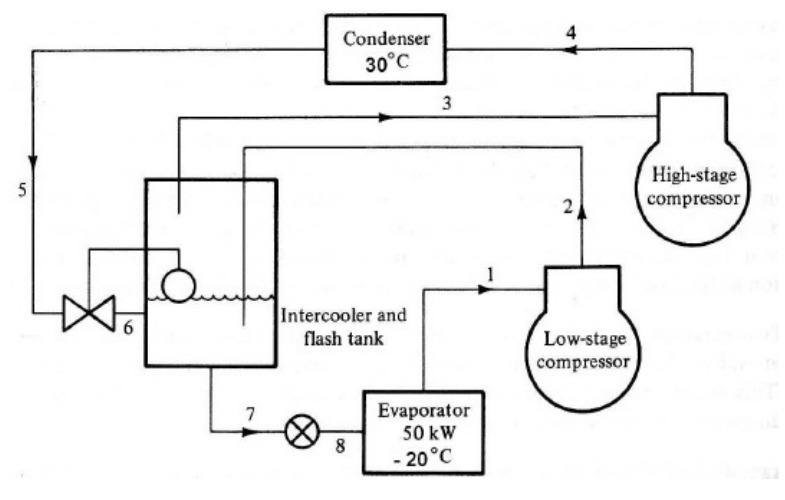
\includegraphics[width=\textwidth]{img/prb-02.jpeg}
      \caption{refrigeration cycle}
      \label{subfig:refrigeration cycle}
  \end{subfigure}
  \hfill
  \begin{subfigure}{0.45\textwidth}
      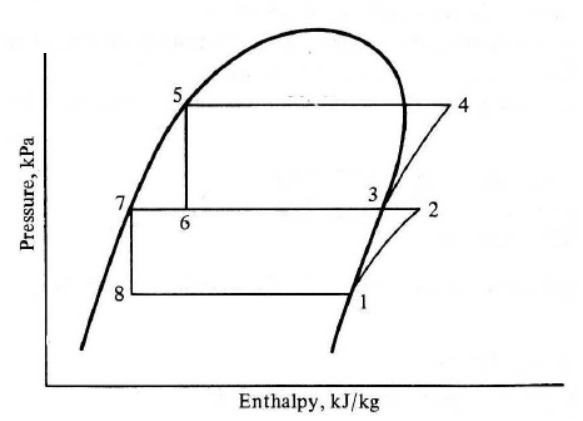
\includegraphics[width=\textwidth]{img/prb-02a.jpeg}
      \caption{p-h diagram}
      \label{subfig:p-d diagram of problem 02}
  \end{subfigure}
  
  \caption{Problem-02 Solution}
  \label{fig:problem 02}
\end{figure}

\begin{multicols}{2}
  Given,\\
  $T_{cond}$ = 30°C \\
  $T_{evap}$ = -20°C \\
  $T_{inter-cooler}$ = 0°C \\
  R.E. = 50 kW \\
  C.O.P. = ? \\
  Data:\\
  $h_1$ = 386.55 kj/kg , $s_1$ = 1.7413 [From table] \\
  $h_2$ = 400 kj/kg [From p-h chart] \\
  $h_3$ = 398.60 kj/kg , $s_3$ = 1.7271 [From table] \\
  $h_4$ = 415 kj/kg [From p-h diagram] \\
  $h_5$ = $h_6$ = 241.72 kj/kg [From table] \\
  $h_7$ = $h_8$ = 200 kj/kg [from table] \\

  \begin{align*}
    \text{Now, } h_6 &= h_7 + x(h_3 - h_7) \\ 
    \Rightarrow 241.72 &= 200 + x (398.60 - 200) \\
    \Rightarrow x &= 0.21  
  \end{align*}

  
  \begin{align*}
    \text{Again, } R.E. &= \dot{m} (1-x)(h_1 - h_8) \\ 
    \Rightarrow 50 &= \dot{m} \times 0.79 \times (386.55 - 200) \\
    \Rightarrow \dot{m} &= 0.339  
  \end{align*}

$$W_{1-2} = \dot{m}(1-x) (h_2-h_1) = 4.29 KW$$
$$W_{3-4} = \dot{m} (h_4-h_3) = 6.80 KW$$
$$C.O.P. = \frac{R.E.}{W_{1-2} + W_{3-4}} = 4.50 KW$$
\end{multicols}

\subsubsection*{Problem-03}
Do the same problem for the single stage refrigeration system
\subsubsection*{Solution}
\begin{multicols}{2}
  Given,\\
  $T_{cond}$ = 30°C \\
  $T_{evap}$ = -20°C \\
  R.E. = 50 kW \\
  C.O.P. = ? \\
  Data:\\
  $h_1$ = 386.55 kj/kg , $s_1$ = 1.7413 [From table] \\
  $h_2$ = 420 kj/kg [From p-h chart] \\
  $h_3$ = $h_4$ = 241.72 kj/kg [From table] \\

  \begin{align*}
    \text{Again, } R.E. &= \dot{m} (h_1 - h_4) \\ 
    \Rightarrow 50 &= \dot{m} \times (386.55 - 241.72) \\
    \Rightarrow \dot{m} &= 0.345  
  \end{align*}

  $$W_{1-2} = \dot{m}(h_2-h_1) = 11.54 \, KW$$
  $$C.O.P. = \frac{R.E.}{W_{1-2}} = 4.33 \, KW$$

\end{multicols}
\pagebreak
\section{Lecture 4: 2 compressor \& 2 evaporator}
\hfill Date: 17/07/2023

\begin{figure}[H]
  \centering
  
  \begin{subfigure}{0.3\textwidth}
      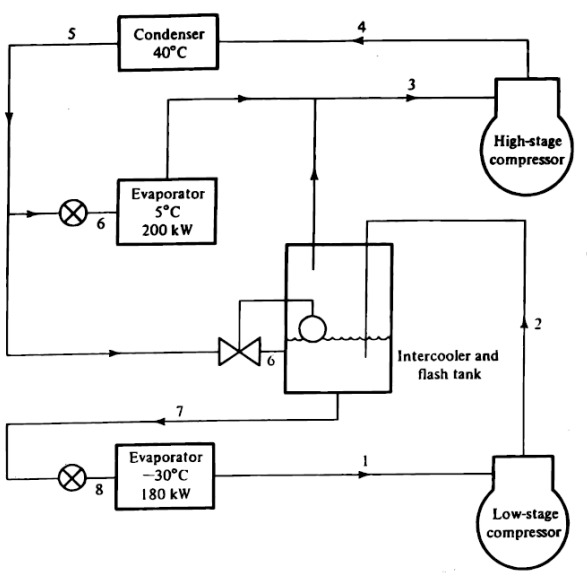
\includegraphics[width=\textwidth]{img/two_com_2_evap.jpeg}
      \caption{2 compressor and 2 evaporator}
      \label{subfig:2_compressor_2_evaporator}
  \end{subfigure}\hfill
  \begin{subfigure}{0.3\textwidth}
      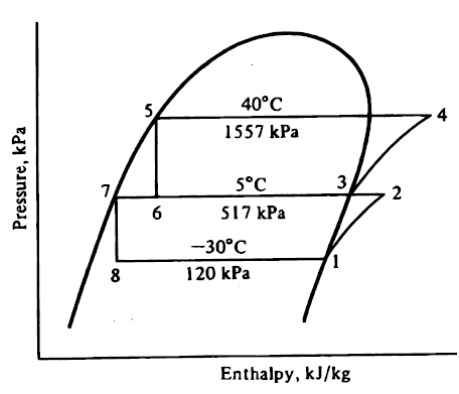
\includegraphics[width=\textwidth]{img/two_com_2_evap_phase_dia.jpeg}
      \caption{Phase diagram}
      \label{subfig:Phase_diagram}
  \end{subfigure}\hfill
  \begin{subfigure}{0.3\textwidth}
      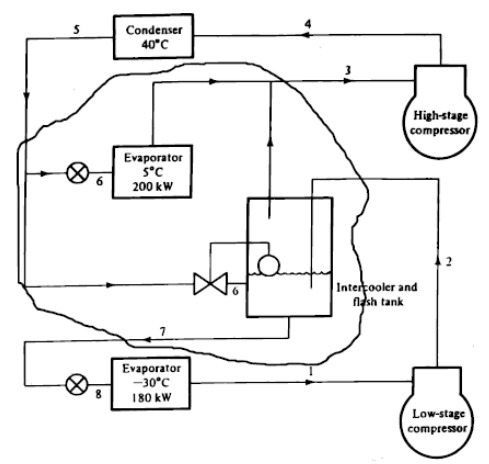
\includegraphics[width=\textwidth]{img/two_com_2_evap_phase_dia_control_volume.jpeg}
      \caption{Control volume approach}
      \label{subfig:Control_volume_approach}
  \end{subfigure}

  \caption{Two compressor and two evaporator problem}
  \label{fig:2-c-2-e} 
\end{figure}
\subsubsection*{Solution:}
\begin{multicols}{2}
  Here, \\
  $m_1 = m_2 = m_7 = m_8$ \\
$m_3 = m_4 = m_5$ \\

\textbf{Reading the properties:}
\begin{align*}
  &h_1 = 380.32 \, \text{kj/kg}, s_1 =  1.7515 \\
  &h_2 = 405 \, \text{kj/kg},  s_2 = 1.7515  \\
  &h_3 = 401 \, \text{kj/kg}, s_3 = 1.7250 \\
  &h_4 = 404 \, \text{kj/kg} \\
  &h_5 = 256 \, \text{kj/kg} \\
  &h_7 = h_8 = 206 \, \text{kj/kg} \\
\end{align*}

Now, Refrigetation effect, R.E.: 
\begin{align*}
  &m_1 (h_1-h_8) = 180 \, kW\\
  &m_1 = 1.03 \, kg/s 
\end{align*}

Here, In intercooler, $m_2$ \& $m_5$ enters and $m_3$ \& $m_7$ exits. We are trying to avoid $m_6$ for simplicity. 

So, we found: \\
$$m_2h_2 + m_5h_5 + 200 = m_3h_3 + m_7h_7$$
As, $m_1 = m_2 = m_7$ and $m_3 = m_5$,by solving,\\
$$m_3 = 2.793 \, kg/s$$

$$W_{1-2} = m_1 (h_2-h_1) = 25.4204 \, kW$$ 
$$W_{3-4} = m_3 (h_4-h_3) = 8.375 \, kW$$ 
$$C.O.P. = \frac{R.E.}{W_{1-2} + W_{3-4}} = 5.326 $$
  
\end{multicols}

\subsubsection*{Some others important parameters:}
\begin{itemize}
  \item $$EER = \frac{\text{R.E. in BTU/hr}}{\text{Power Required in W}}$$
  \item $$ kW/ton = \frac{3.516}{C.O.P.}$$
  \item $$ EER \times kW/ton = 12 $$
\end{itemize}

\pagebreak

\section{Lecture 5: Cooling Load Estimation Using CLTD/CLF Method}
\hfill Date: 24/07/2023

\begin{figure}[H]
  \begin{center}
    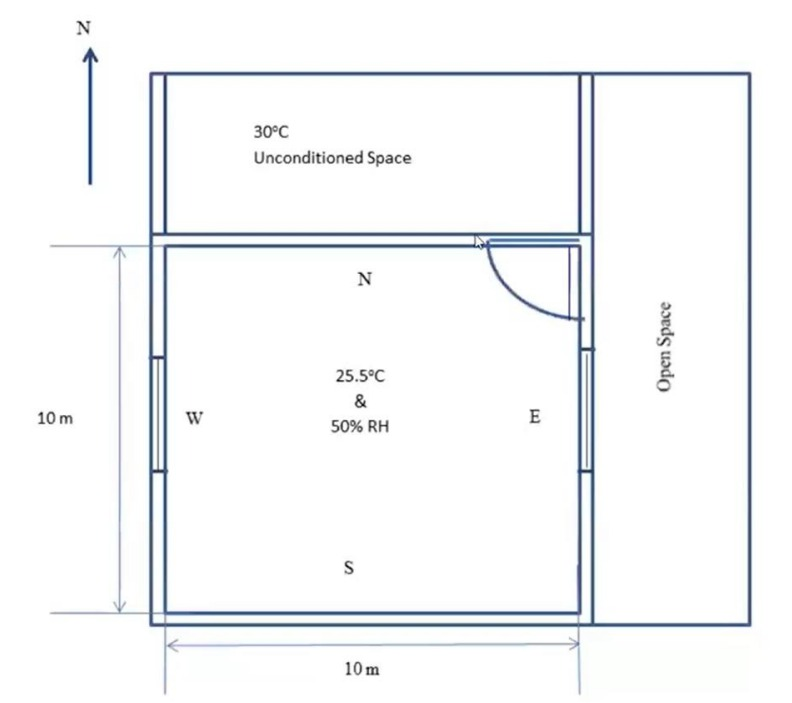
\includegraphics[width=\columnwidth]{img/cooling_load.jpeg}
    \caption{CAD model of room for cooling load estimation}
  \end{center}
\end{figure}

\begin{multicols}{2}
  \begin{enumerate}
    \item Normally at 5-6 pm, temperatures are high. Also in April/May, temperatures are high. So, we have to design for the worst case scenario.
    \item Room height: 3.0 m
    \item West \& South Walls: Metal curtain wall, construction type G with 75 mm insulation, sunlit, dark color. 
    \item Partition walls (North \& East): 127 mm brick with 25 mm plaster on both sides. 
    \item Roof: Type 4, 50 mm insulation without suspended ceiling 
    \item Window: 6 $m^2$ on west \& east side.\\U = 2.86 $W/m^2-k$\\- 13 mm thickness\\- Light construction  
    \item No heat transfer through floor
    \item Air exchange rate: 1.0 / h \\- ($10 \times 10 \times 3 = 300 \, m^3/h$)
    \item Light \& Occupants from 8 am to 6 pm. 
    \item Average light density: 25 $W/m^2$, flouroscent light\\- $25 \times \text{Area of Base} = 2500$
    \item 5 Occupants seated, using 1 computer. 
    \item Door in North wall: Door size: $2 m \times 1 m$, 25 mm thick, hard wood. 
  \end{enumerate}

  \subsection*{Heat Conduction through Surface}
  \begin{enumerate}
    \item Conduction Through Shaded Partition/Surface:\\
    $$Q = U.A.TD$$ 
    \item Conduction Through Sunlit Surface:\\
    $$Q = U.A.CLTD$$
  \end{enumerate}
  \begin{itemize}
    \item $U \rightarrow$ Overall heat conductance ($W/m^2-k$)
    \item $TD \rightarrow$ Temperature difference accross the surface ($^\circ C$)
    \item $CLTD \rightarrow$  Cooling load temperature difference ($^\circ C$)
    \item $U = 1/R_{th}$ 
    \item $R_{th} = R_{o} + R + R_{i}$
  \end{itemize}
\end{multicols}

\vspace*{1cm}
  \subsection*{\# Roof}
  \begin{itemize}
    \item Type: Type 4, 50 mm insulation without suspended ceiling
    \item Read data from \textbf{Table 12(a)} 
    \item Layers for type-4 : $A0 - E2 - E3 - B5 - C12 - E0$
    \item Here, 50 mm insulation not available on type 4. That's why we have to switch from $B5$ to $B6$. 
    \item So, we have to calculate for: $A0 - E2 - E3 - B6 - C12 - E0$
    \item Read the resistance of the layers from \textbf{Table-16}
  \end{itemize}

  \begin{figure}[H]
    \begin{center}
      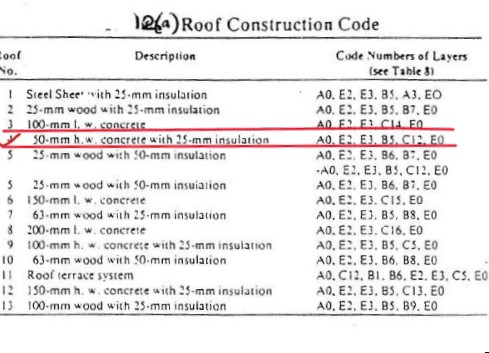
\includegraphics[width=\columnwidth]{img/roof.jpeg}
      \caption{Table 12(a) : Type 4}
    \end{center}
  \end{figure}

  \subsubsection*{Calculation for Roof:}
  \begin{table}[H]
    
    \renewcommand{\arraystretch}{1.5}
    \begin{tabular*}{\textwidth}{@{\extracolsep{\fill}}|c|c|c|c|c|c|c|c|}
        \hline
        Layer & A0 & E2 & E3 & B6 & C12 & E0 & Total \\
        \hline
        $R_{th}$ & 0.059 & 0.099 & 0.050 & 1.173 & 0.029 & 0.121 & 1.581 \\
        \hline
    \end{tabular*}
    \caption{Resistance of all layers for roof.}
    \label{tab:roof}
\end{table}
Now, $R_{th} = 1.581$, \\so, $U = 1/R_{th} = 0.653$

\vspace*{1cm}
\subsection*{\# South \& West Wall}
\begin{itemize}
  \item Type: Metal curtain wall, construction type G with 75 mm insulation, sunlit, dark color.
  \item Read data from \textbf{Table-14}
  \item Layers: $A0 - A3 - B12 - A3 - E0$
  \item Read resistance value from \textbf{Table-16}
\end{itemize}

\begin{figure}[H]
  \begin{center}
    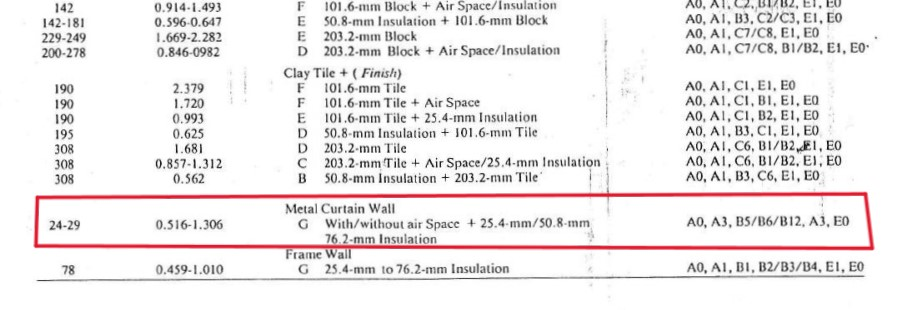
\includegraphics[width=\columnwidth]{img/sw_walls.jpeg}
    \caption{Table 14 : Type G}
  \end{center}
\end{figure}
\subsubsection*{Calculation for South \& West Walls:}
\begin{table}[H]    
  \renewcommand{\arraystretch}{1.5}
  \begin{tabular*}{\textwidth}{@{\extracolsep{\fill}}|c|c|c|c|c|c|c|}
      \hline
      Layer & A0 & A3 & B12 & A3 &  E0 & Total \\
      \hline
      $R_{th}$ & 0.059 & 0 & 1.76 & 0 & 0.121 & 1.94 \\
      \hline
  \end{tabular*}
  \caption{West and South walls.}
  \label{tab:west-south-walls}
\end{table}
Now, $R_{th} = 1.94$, \\so, $U = 1/R_{th} = 0.52$

\vspace*{1cm}
\subsection*{\# North \& East Wall (Partition Wall)}
\begin{itemize}
  \item 127 mm brick with 25 mm plaster on both sides.
  \item Read resistance from \textbf{Table-16}
  \item Here, 127 mm brick not available. So, we will take $C4: 100 $ mm brick to calculate $k = 0.727$, then calculate the resistance for 127 mm brick with the same $K$ values. 
  \item Also 25 mm plaster not availble. We will take $E1 : 20 mm$, then by the value of $k=0.7277$, will calculate resistance for 25 mm plaster.
\end{itemize}
\begin{figure}[H]
  \begin{center}
    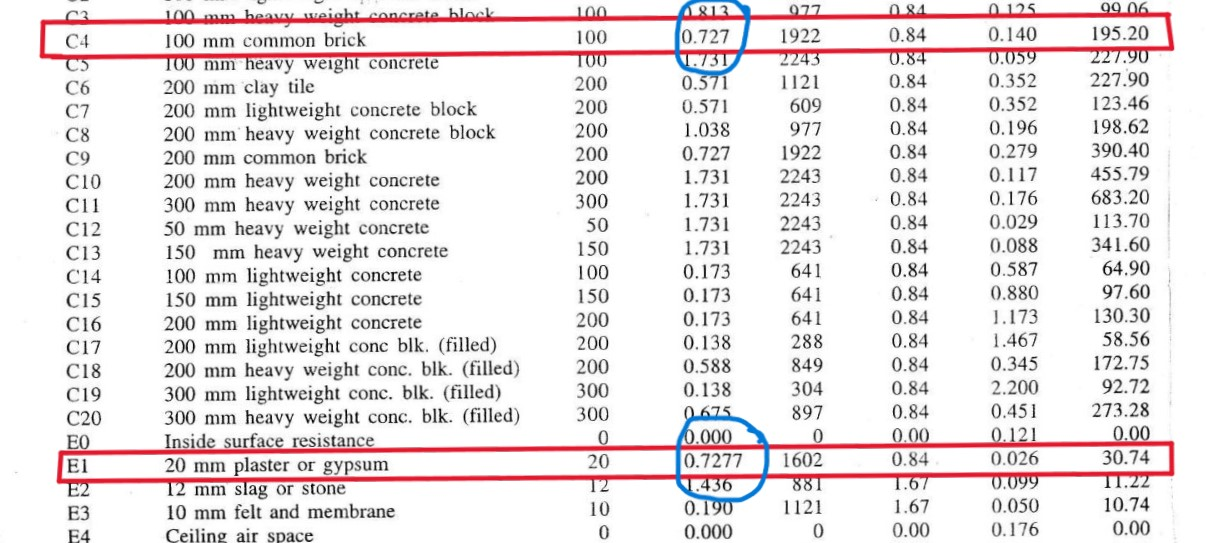
\includegraphics[width=\columnwidth]{img/partition.jpeg}
    \caption{Table 16 : For partition walls}
  \end{center}
\end{figure}

\subsubsection*{Calculation for North \& East Wall:}
\begin{itemize}
  \item $R_{th} = R_o + R_1 + R_2 + R_3 + R_i $
  \item Outside ($R_0$) : A0 = 0.059 
  \item 25 mm Plaster ($R_1, R_3$) : For E1 20 mm plaster, k = 0.7277, now $R_1 = R_3 = L/k = 0.025/0.7277 = 0.0343$ 
  \item 127 mm Brick ($R_2$) : For C4 100 mm brick, k = 0.727, now $R_2 = L/k = 0.127/0.727 = 0.175$
  \item Inside ($R_i$) : E0 = 0.121
  \item Total ($R_{th}$) = 0.059 + 0.0343 + 0.175 + 0.0343 + 0.121 = 0.4236
  \item $U = 1/R_{th} = 2.36$ 
\end{itemize}

\vspace*{1cm}
\subsection*{\# Door}
\begin{itemize}
  \item Door size: $2 m \times 1 m$, 25 mm thick, hard wood
  \item Read data from \textbf{Table-17.6}
  \item Hard wood, Oak, k= 0.16. $R_d = L/k = 0.025/0.16 = 0.156$
  \item $R_{th} = R_o + R_d + R_i = 0.059 + 0.156 + 0.121 = 0.336$
  \item $U = 2.98$
\end{itemize}

\begin{figure}[H]
  \begin{center}
    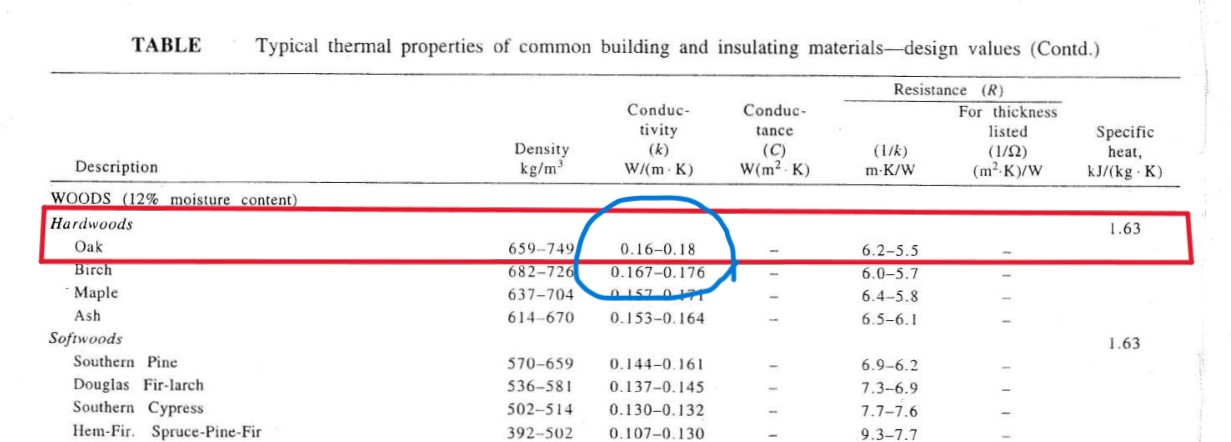
\includegraphics[width=\columnwidth]{img/door.jpeg}
    \caption{Table 17.6 : For door (hardwood, i.e.: Oak)}
  \end{center}
\end{figure}
\vspace*{1cm}

\subsection*{Heat Conduction through Partition walls/glasses}
\begin{figure}[H]
  \begin{center}
    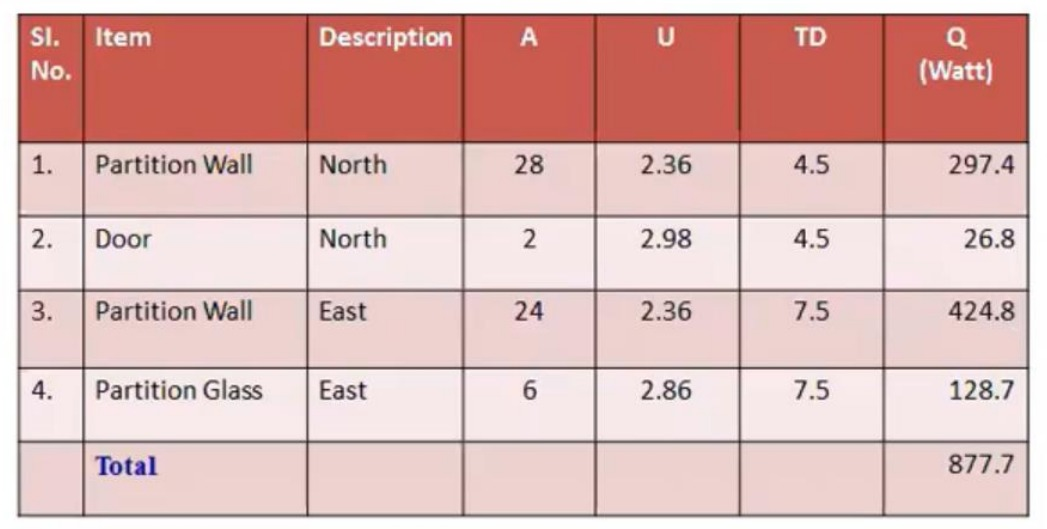
\includegraphics[width=\columnwidth]{img/head_conduction.jpeg}
    \caption{Heat Conduction through Partition walls/glasses}
  \end{center}
\end{figure}

\begin{itemize}
  \item For 1 \& 2: $TD = T_o - T_i = 30 - 25.5 = 4.5$
  \item For 3 \& 4: $TD = T_{o,max} - T_i = 33 - 25.5 = 7.5$ [From table-9: $T_{o,max} = 33$ for BD]
  \item For 1: A = Northern wall - Door = $(10 \times 3) - (2 \times 1) = 28$ 
  \item For 3: A = Eastern wall - Window = $30 - 6 = 24$
\end{itemize}
\begin{figure}[H]
  \begin{center}
    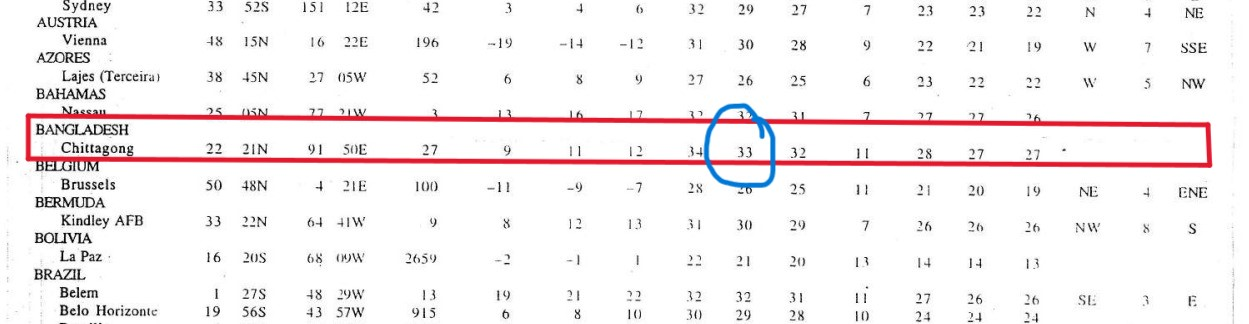
\includegraphics[width=\columnwidth]{img/t_o_max.jpeg}
    \caption{$T_{o,max}$ from table-9 (design dry bulb - 2.5\%)}
  \end{center}
\end{figure}
\end{document}
